\title{Math 239 Fall 2023 Tutorial Answers Week 8}

\date{2023 Nov. 9/10}
\maketitle

\begin{enumerate}
    \question{Exotic Cubes}
    \begin{enumerate}
        \item There are $3^2 = 9$ vertices in this graph ($m^n$ in general).
\begin{center}
    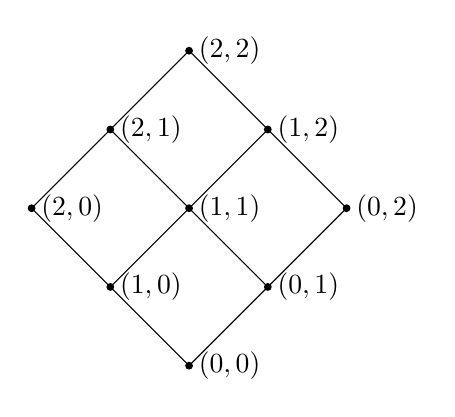
\begin{tikzpicture}
        \coordinate[label = right:{$(0,0)$}] (00) at (0,-2);
        \coordinate[label = right:{$(0,1)$}] (01) at (1,-1);
        \coordinate[label = right:{$(0,2)$}] (02) at (2,0);
        \coordinate[label = right:{$(1,0)$}] (10) at (-1,-1);
        \coordinate[label = right:{$(1,1)$}] (11) at (0,0);
        \coordinate[label = right:{$(1,2)$}] (12) at (1,1);
        \coordinate[label = right:{$(2,0)$}] (20) at (-2,0);
        \coordinate[label = right:{$(2,1)$}] (21) at (-1,1);
        \coordinate[label = right:{$(2,2)$}] (22) at (0,2);
        
        \node at (00)[circle,fill,inner sep=1pt]{};
        \node at (01)[circle,fill,inner sep=1pt]{};
        \node at (02)[circle,fill,inner sep=1pt]{};
        \node at (10)[circle,fill,inner sep=1pt]{};
        \node at (11)[circle,fill,inner sep=1pt]{};
        \node at (12)[circle,fill,inner sep=1pt]{};
        \node at (20)[circle,fill,inner sep=1pt]{};
        \node at (21)[circle,fill,inner sep=1pt]{};
        \node at (22)[circle,fill,inner sep=1pt]{};

        \draw (00) -- (10) (00) -- (01);
        \draw (10) -- (20) (10) -- (11);
        \draw (01) -- (11) (01) -- (02);
        \draw (20) -- (21);
        \draw (11) -- (21) (11) -- (12);
        \draw (02) -- (12);
        \draw (21) -- (22);
        \draw (12) -- (22);
    \end{tikzpicture}
\end{center}
        \item $G_p$ is always bipartite. This is given by the usual bipartition $V_1 \sqcup V_2$ where $V_1$ has all vertices with even coordinate sum and $V_2$ has all vertices with odd coordinate sum. Since two vertices are adjacent only their coordinate sums differ by one, this is a good bipartition.
        \item The degree of a vertex is maximized if $v \pm e_j$ exists for all $e_j$, ie if we can change each coordinate by $1$ while keeping our coordinates in $\{ 0 , \cdots, m-1 \}$. It follows that the maximum degree is $2n$ (attained by, for example, the point $(1, \cdots, 1)$). Minimum degree is attained when we have as few directions to move in general. This happens when we cannot remove or add $1$ from as many coordinates as possible. Since we can still either add or remove from one coordinate then the minimum degree is $n$ (for example the point $(0,\cdots, 0)$).
        \item I would recommend not writing this part of the question. From my scratch-work we should have
        \begin{align*}
            |E| = \frac{1}{2} \sum_{j=0}^n (2n - j) (m-2)^{n-j} 2^j \binom{n}{j}.
        \end{align*}
        I am not sure if this simplifies in any nice way. For more details on my thinking consult the bonus questions document.
    \end{enumerate}
    % \question{Complete $k$-partite Graphs} This requires some thinking and may be too hard for some people. You may consider skipping the proof of part b) and just state the result.
    % \begin{enumerate}
    %     \item This comes from using the HL. Note that there are $p$ vertices with degree $2n-p$ and $2n-p$ vertices with degree $p$. By the HL this becomes
    %     \begin{align*}
    %         2 |E| &= \sum_v \deg (v) = p(2n-p) + (2n-p) p\\
    %         \implies |E| &= p(2n-p) = np - p^2.
    %     \end{align*}
    %     Treating this as a function depending on $p$ gives us a usual calculus maximization problem. Differentiating with respect to $p$ and setting to $0$ gives $p=n$, which gives the maximum number of edges occurring in $K_{n,n}$. From the above this has $n^2$ edges.
    %     \item Think about a complete $k$-partite graph. Then each vertex in the part $V_j$ has degree $kn - |V_j|$. Then using the HL gives that
    %     \begin{align*}
    %         |E| = \frac{1}{2} \sum_{i=1}^k |V_i| (kn - |V_i|).
    %     \end{align*}
    %     Now we will show that the maximum happens when $|V_i| = n$ (ie the vertices are split evenly) for all $i$. Assume for a contradiction that the maximum number of edges occurs for some partition where not every part has $n$ vertices. Then let $A$ denote the part with the most vertices and $B$ denote the part with the least vertices. Then since not every part has $n$ vertices then $|A| - |B| \geq 2$ (otherwise then the average of the parts will be some fraction, and so certainly the sum of the parts will not be $kn$). Now consider taking a vertex in $A$ and moving it to $B$. The number of edges between $A \cup B$ and the other parts will not change, so we must only show that the number of edges between $A$ and $B$ will increase. But this is true from part a), since the number of edges between $A$ and $B$ is maximized when their sizes are the same or close to being the same. It follows that we can find a partition that has more edges in it, and so our assumption that not every part had $n$ vertices was erroneous. Thus the maximum number of edges occurs when $|V_j| = n$ for all $j = 1 , \cdots, k$, and so the maximum number of edges is
    %     \begin{align*}
    %         |E| &= \frac{1}{2} \sum_{i=1}^k n (kn - n)\\
    %         &=\frac{k(k-1)}{2} n^2\\
    %         &= \binom{k}{2} n^2.
    %     \end{align*}
    % \end{enumerate}
    
    \newpage
    \question{Find the Mistake} To see the non-theorem is false observe that the graph consisting of two disjoint three cycles satisfies the theorem conditions but does not contain a cycle of length four. The non-proof falsely assume that all graphs satisfying the statement can be constructed by taking a graph that does and adding a new vertex. This is not true. To see this consider two disjoint four cycles as a graph. This graph satisfies that statement and cannot be constructed in this manner.
    \\
    \textbf{Theorem:} If $G$ is a graph with $|V(G)|\geq 3$ and minimum degree at least $2$, then $G$ contains a cycle. 
    \\
    \textbf{Proof:} Suppose not. Then there exists a graph $G$ such that $|V(G)|\geq 3$, the minimum degree of $G$ is at least $2$ and $G$ does not contain a cycle. Since $G$ does not contain a cycle $G$ is a tree. Since $G$ is a tree $G$ has a leaf, which is a vertex of degree one. A contradiction. Hence the theorem holds. 

    \newpage
    \question{Pr{\"u}fer Codes} 
    \begin{enumerate}
        \item The codes are 
        
        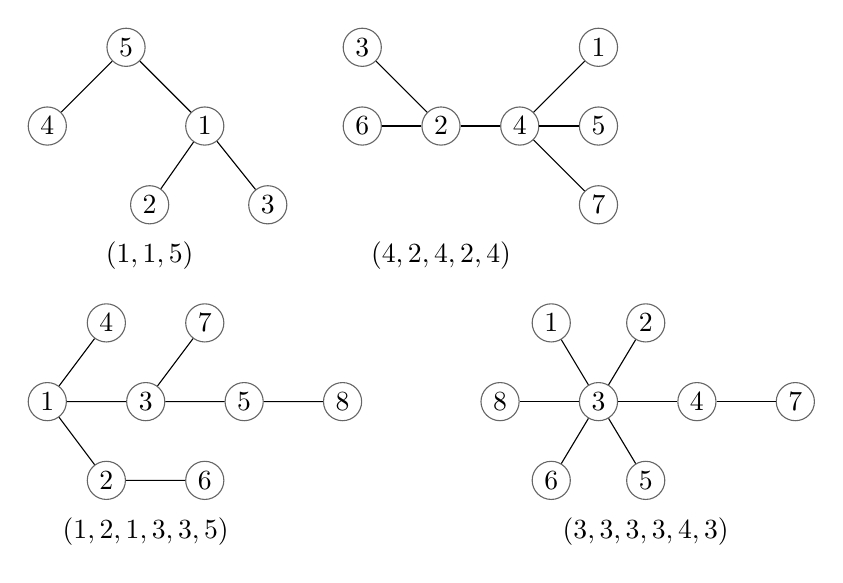
\begin{tikzpicture}[shorten >=1pt,->]
  \tikzstyle{vertex}=[circle,draw=black!60,minimum size=12pt,inner sep=2pt]
  \node[vertex] (G_4) at (-1,-1) {4};
  \node[vertex] (G_5) at (0,0)   {5};
  \node[vertex] (G_1) at (1,-1)  {1};
  \node[vertex] (G_2) at (0.3,-2)  {2};
  \node[vertex] (G_3) at (1.8,-2)  {3};
  \draw (G_4) -- (G_5) -- (G_1) -- (G_2) -- cycle;
  \draw (G_1) -- (G_3) -- cycle;
  \node [below=0.35cm] at (G_2)
        {$(1, 1, 5)$};

\node[vertex] (G_6') at (3,-1) {6};
\node[vertex] (G_3') at (3,0) {3};
  \node[vertex] (G_2') at (4,-1)   {2};
  \node[vertex] (G_4') at (5,-1)  {4};
  \node[vertex] (G_1') at (6,0)  {1};
  \node[vertex] (G_5') at (6,-1)  {5};
  \node[vertex] (G_7') at (6,-2)  {7};
  \draw (G_6') -- (G_2') -- (G_4') -- (G_5') -- cycle;
  \draw (G_4') -- (G_1') -- cycle;
  \draw (G_3') -- (G_2') -- cycle;
  \draw (G_4') -- (G_7') -- cycle;
  \node [below=1.35cm] at (G_2')
        {$(4, 2, 4, 2, 4)$};

  \node[vertex] (G_4'') at (-0.25,-3.5) {4};
  \node[vertex] (G_1'') at (-1,-4.5)   {1};
  \node[vertex] (G_2'') at (-0.25,-5.5)  {2};
  \node[vertex] (G_6'') at (1,-5.5)  {6};
  \node[vertex] (G_3'') at (0.25,-4.5)  {3};
  \node[vertex] (G_7'') at (1,-3.5)  {7};
  \node[vertex] (G_5'') at (1.5,-4.5)  {5};
  \node[vertex] (G_8'') at (2.75,-4.5)  {8};
  \draw (G_1'') -- (G_4'') -- cycle;
  \draw (G_6'') -- (G_2'') -- (G_1'') -- (G_3'') -- (G_5'') -- (G_8'') -- cycle;
  \draw (G_3'') -- (G_7'') -- cycle;
  \node [below=1.35cm] at (G_3'')
        {$(1, 2, 1, 3, 3, 5)$};

  \node[vertex] (H_3) at (6,-4.5) {3};
  \node[vertex] (H_1) at (5.4,-3.5)   {1};
  \node[vertex] (H_2) at (6.6,-3.5)   {2};
  \node[vertex] (H_4) at (7.25,-4.5)  {4};
  \node[vertex] (H_7) at (8.5,-4.5)  {7};
  \node[vertex] (H_8) at (4.75,-4.5)  {8};
  \node[vertex] (H_6) at (5.4,-5.5)   {6};
  \node[vertex] (H_5) at (6.6,-5.5)   {5};
  \draw (H_8) -- (H_3)  -- (H_4)  -- (H_7) -- cycle;
  \draw (H_1) -- (H_3)  -- (H_5)  -- cycle;
  \draw (H_2) -- (H_3)  -- (H_6)  -- cycle;
  \node [below=0.35cm] at (H_5)
        {$(3, 3, 3, 3, 4, 3)$};
    
\end{tikzpicture}
    \item Suppose we have sequence $(\sigma_1, \dots, \sigma_{n-2})$. Start with an empty graph on $n$ vertices. 
    
    The inverse algorithm is roughly:
    \begin{enumerate}
    \item Let $x$ be the largest number in $\{1, \dots, n\}$ that doesn't appear in $(\sigma_k, \dots, \sigma_{n-2})$
    \item While the sequence is non-empty, repeat the following:
        \begin{enumerate}
            \item Let $v$ be the lowest number of $\{1, \dots, n\}$ that doesn't appear in $(\sigma_k, \dots, \sigma_{n-2})$ and that has no edges in our graph.
            \item Draw an edge between $v$ and $\sigma_k$.
            \item Delete $\sigma_{k}$ from the beginning of the sequence. 
        \end{enumerate}
    \item Draw an edge between $x$ and $\sigma_{n-2}$.
    \end{enumerate}
    \item If we count the number of possible sequences of length $n-2$ of $\{1, \dots, n\}$, we get $n^{n-2}$. We take as given that we have a bijection, so that's the number of labeled trees.

    \item \textbf{Bonus:} This will be a bit trickier to prove, but we have surjectivity from part (b). For injectivity it's an induction argument but for the induction hypothesis, you need to weaken the constraint that elements are strictly from $\{1, \dots, n\}$ and instead just assume you have $n$ elements of $\mathbb{N}$. There's also an argument that needs to be made regarding the relationship between degree and how many times the vertex appears in the sequence. 
    \end{enumerate}

    \newpage
    \question{Spanning Tree} First, assume that $e=\{v,w\}$ is a bridge in a connected graph $G$. Arguing for a contradiction, suppose that $T$ is a spanning tree of $G$ that does that not contain $e$. Since $T$ is a spanning subgraph of $G$, both $v$ and $w$ are vertices of T. Since $T$ is a tree, there is a unique path $P$ in $T$ from $v$ to $w$ (Lemma 5.1.3 in IC notes). But now $C=T\cup\{e\}$ is a cycle in $G$ that contains the edge $e$. Non of the edge in a cycle can be a bridge (Lemma 4.10.3 in IC notes), so $e$ is not a bridge. This contradiction shows that if $e$ is a bridge then $e$ is contained in every spanning tree of $G$.

    Conversely, assume that $e$ is not a bridge. Then $H = G \setminus e$ is still connected. Every connected graph has a spanning tree (Theorem 5.2.1 in IC notes), then the graph $H$ has a spanning tree $T$. Since $H$ is a spanning subgraph of $G$, this spanning tree $T$ of $H$ is also a spanning tree of $G$. Since $T$ does not contain $e$, this completes the proof.
    
\end{enumerate}